\section{Auswertung}
\label{sec:Auswertung}

\subsection{Heizrate}

Um zunächst die Messungen zu unterscheiden werden die Heizraten bestimmt. Sie ergeben sich aus dem Differenzquotienten der Temperatur $T$ pro Zeit $t$.
Durch Auftragen von $T$ gegen $t$ wird eine lineare Ausgleichsrechnung möglich, dessen Steigung die Heizrate $b_i$ beträgt (vgl. Abb. \ref{fig:heiz}).
Die dazugehörigen Ergebnisse sind
\begin{align}
    b_1 &= \qty{1.9518(23)}{\kelvin\per\minute} & T_{0,1} &= \qty{223.11(8)}{\kelvin} \\
    b_2 &= \qty{1.4508(19)}{\kelvin\per\minute} & T_{0,2} &= \qty{221.72(9)}{\kelvin}.
\end{align}
Die Indizes $i = 1,2$ stehen dabei für die Nummer der Messung.

\begin{figure}
    \centering
    \includegraphics[width=0.8\linewidth]{scripts/build/Heizrate.pdf}
    \caption{Temperatur-Zeit Diagramm der beiden Messungen.}
    \label{fig:heiz}
\end{figure}

\subsection{Untergrund}
Die aufgenommenen Messwerte enthalten einen exponentiellen Untergund, der die Messung verfälscht.
Dieser lässt sich betrachten indem man eine Ausgleichsrechnung der anfänglichen Messwerte nahe $I=0$ und der Stützstellen nach kompletten Abklingen des Depolarisationsstroms
an die Funktion
\begin{equation}
    bgr(T) = c \cdot \exp(-dT)
\end{equation}
durchführt. Dies wird mithilfe der $curve fit$ Funktion aus der Python-Bibliothek SciPy\cite{scipy} umgesetzt. 

Die berechneten Parameter sind bei der ersten Messung
\begin{align}
    c_1 = \qty{1.147(474)e-4}{\ampere} & d_1 = \qty{4460(112)}{\per\kelvin}.
\end{align}
Durch Abziehen des Untergrundes ergeben sich somit die wirklichen korrigierten Messwerte.
In \autoref{fig:bgr1} ist dies graphisch dargestellt.
\begin{figure}
    \centering
    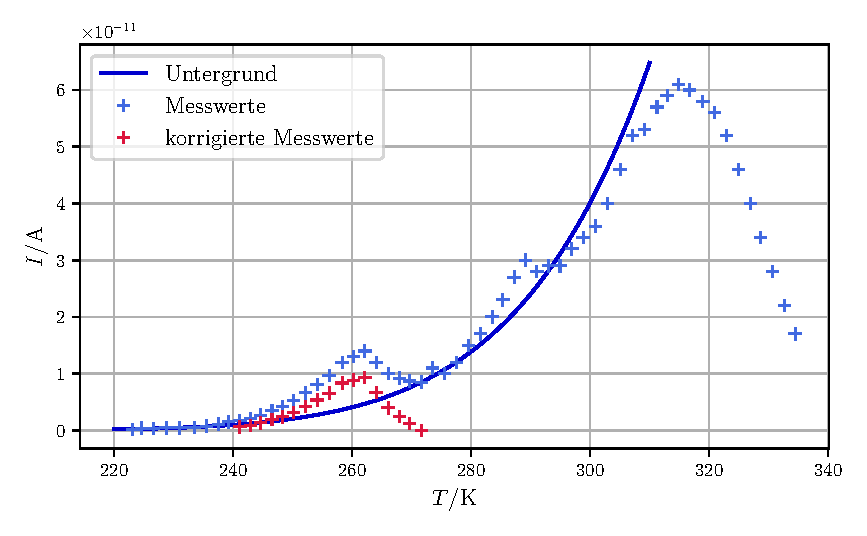
\includegraphics[width=0.8\linewidth]{scripts/build/plot1_bgr.pdf}
    \caption{Untergrundbereinigung der Messung 1.}
    \label{fig:bgr1}
\end{figure}

Bei der zweiten Messung betragen die Parameter
\begin{align}
    c_1 = \qty{2.93(1.45)e-07}{\ampere} & d_1 = \qty{3018(142)}{\per\kelvin}.
\end{align}
Die dazugehörigen Messwerte, sowie Bereinigung, sind in \autoref{fig:bgr2} zu sehen.
\begin{figure}
    \centering
    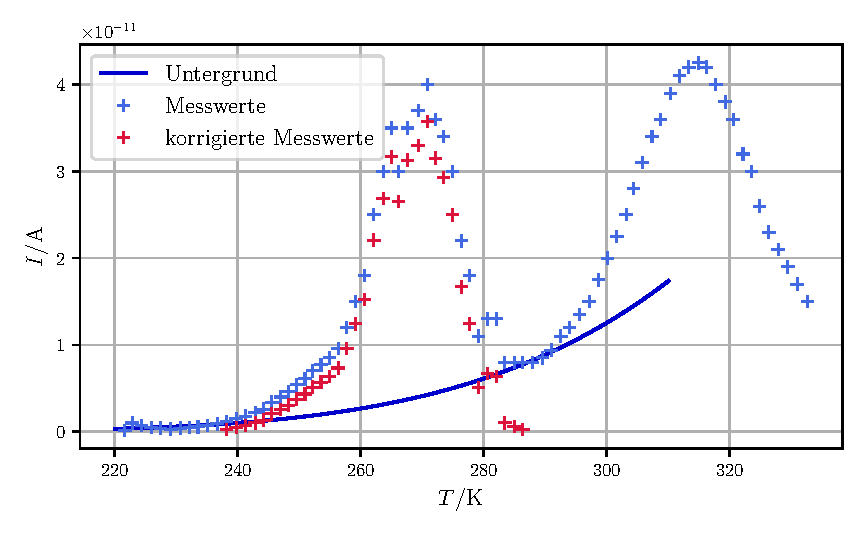
\includegraphics[width=0.8\linewidth]{scripts/build/plot2_bgr.pdf}
    \caption{Untergrundbereinigung der Messung 2.}
    \label{fig:bgr2}
\end{figure}

\subsection{Aktivierungsenergie}
Die linearen Ausgleichrechnungen der Geraden werden im folgenden Unterkapitel mit der Funktion $polyfit$ der Python-Bibliothek numpy\cite{numpy} berechnet.
\subsubsection{Polarisationsansatz}
Zur Bestimmung der Aktivierungsenergie $W$ werden die gemessenen Depolarisationsströme $I(T)$ in den Temperaturintervallen
logarithmisch gegenüber $1/T$ aufgetragen (vgl. Abb. \ref{fig:W1_1} \& \ref{fig:W1_2}). Anschließend können durch eine lineare Ausgleichsrechnung an \autoref{eq:W1}, die Parameter
\begin{align}
    m_1 &= - \frac{W_1}{k_B} = \qty{-7893(472)}{\kelvin} & c_1 &= const = \num{4.97(1.87)} \\
    m_2 &= - \frac{W_2}{k_B} = \qty{-8034(364)}{\kelvin} & c_1 &= const = \num{5.86(1.41)}
\end{align}
berechnet werden. Mit $k_B \approx \qty{8,617e-5}{\electronvolt\per\kelvin}$ folgen daraus
\begin{align}
    W_1 &= \qty{0.680(41)}{\electronvolt} \\
    W_2 &= \qty{0.692(31)}{\electronvolt}.
\end{align}
\begin{figure}
    \centering
    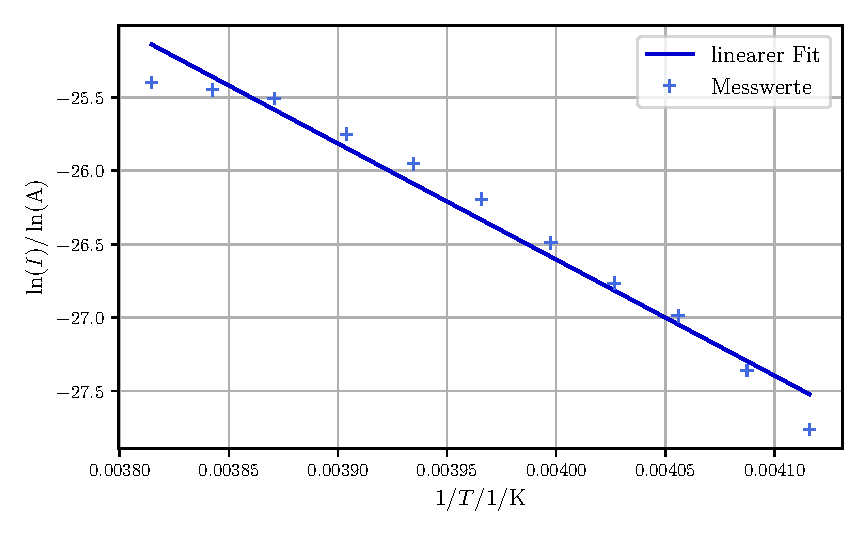
\includegraphics[width=0.8\linewidth]{scripts/build/plot1_1.pdf}
    \caption{Logarithmisches Strom gegen inverse Temperatur Diagramm der Messung 1.}
    \label{fig:W1_1}
\end{figure}
\begin{figure}
    \centering
    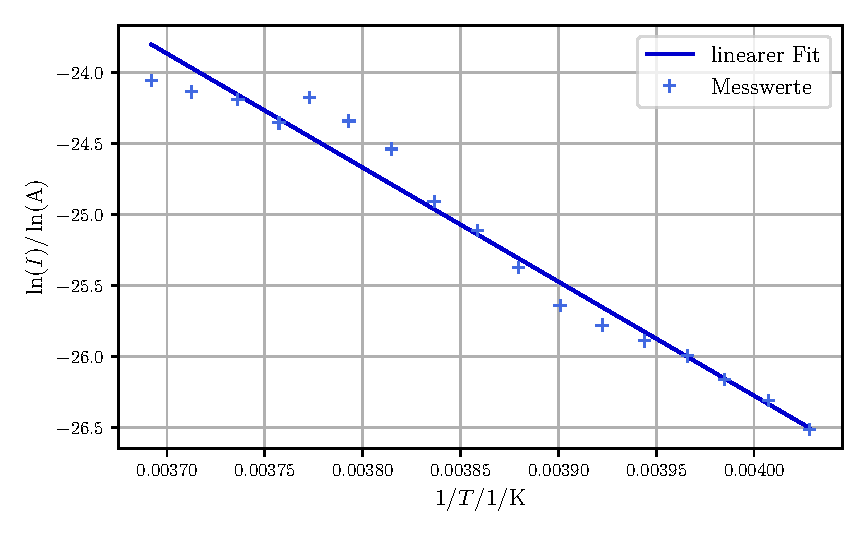
\includegraphics[width=0.8\linewidth]{scripts/build/plot2_1.pdf}
    \caption{Logarithmisches Strom gegen inverse Temperatur Diagramm der Messung 2.}
    \label{fig:W1_2}
\end{figure}

\subsubsection{Stromdichtenansatz}
Durch umstellen von \autoref{eq:Int} zu 
\begin{equation*}
    \ln\left(\frac{\int_{T_0}^{T_{|I=0}} I(T')dT'}{b I(T)}\right) = \frac{W}{k_B}\frac{1}{T} + ln(\tau_0) := m\cdot\frac{1}{T} + y
\end{equation*}
kann nach Auftragen von $\ln\left(\frac{\int_{T_0}^{T_{|I=0}} I(T')dT'}{b I(T)}\right)$ gegen $1/T$ (vgl. Abb. \ref{fig:W2_1} \& \ref{fig:W2_2})
erneut durch eine lineare Ausgleichsrechnung die Aktivierungsenergie berechnet werden.
Hierbei folgte die Integration der bereinigten Kurve mit $scipy.integrate$ der Python-Bibliothek SciPy\cite{scipy}.
Die berechneten Fit-Parameter belaufen sich auf
\begin{align}
    m_1 &= \qty{7893(472)}{\kelvin} & y_1 &= \num{-28.74(1.87)} \\
    m_2 &= \qty{8034(364)}{\kelvin} & y_2 &= \num{-27.92(1.41)} \\
\end{align}
und somit ergibt sich für die Aktivierungsenergien mit $k_B \approx \qty{8,617e-5}{\electronvolt\per\kelvin}$
\begin{align}
    W_1 &= \qty{0.680(41)}{\electronvolt} \\
    W_2 &= \qty{0.692(31)}{\electronvolt}.
\end{align}
\begin{figure}
    \centering
    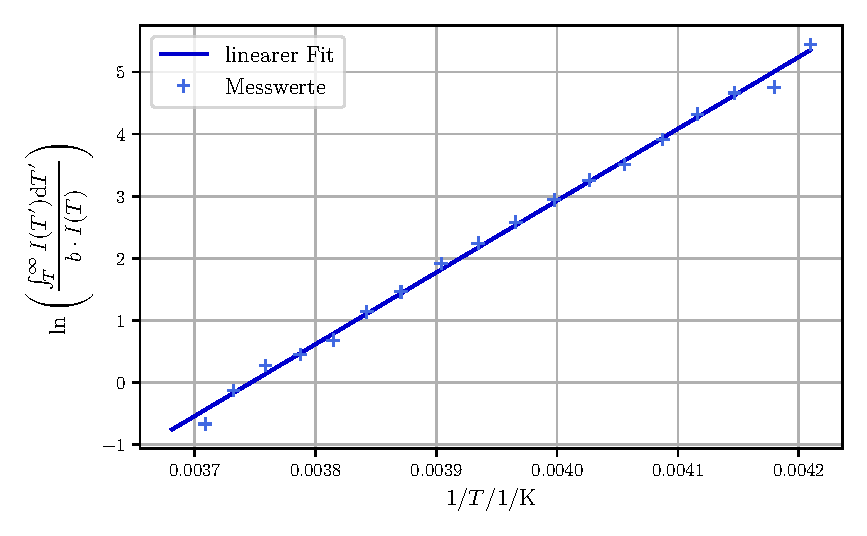
\includegraphics[width=0.8\linewidth]{scripts/build/plot1_2.pdf}
    \caption{Nach Vorschrift integrierte Messwerte der ersten Reihe.}
    \label{fig:W2_1}
\end{figure}
\begin{figure}
    \centering
    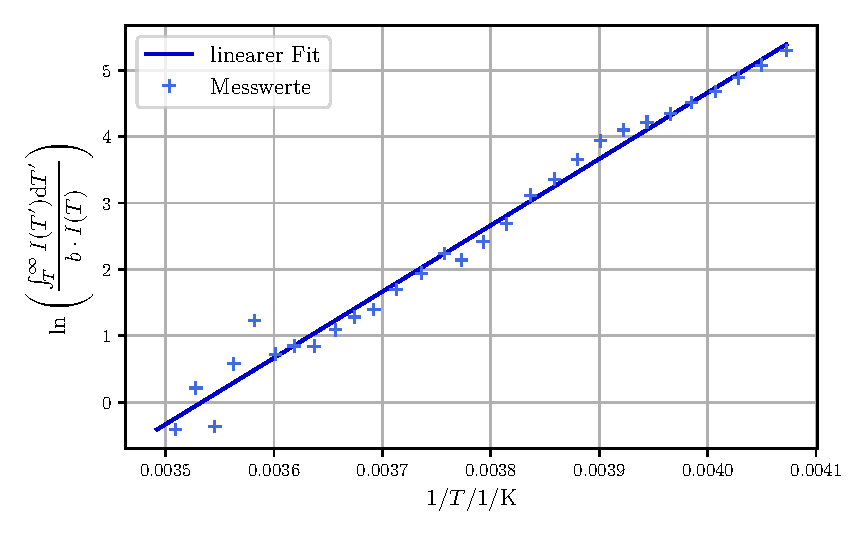
\includegraphics[width=0.8\linewidth]{scripts/build/plot2_2.pdf}
    \caption{Nach Vorschrift integrierte Messwerte der zweiten Reihe.}
    \label{fig:W2_2}
\end{figure}

\subsection{Relaxationszeit}
\subsubsection{Charakteristische Relaxationszeit}
Die Temperaturen der maximalen Depolarisationsströme sind:
\begin{align}
    T_{max,1} &= \qty{262.15}{\kelvin} \\
    T_{max,2} &= \qty{270.85}{\kelvin}
\end{align}
Nach \autoref{eq:relax} sind mit den Aktivierungsenergien der Auswertung des Polarisationsansatzes
die charakteristischen Relaxationszeiten:
\begin{align}
    \tau_{1,1} &= \qty{2.25(4.18)e-11}{\second}\\
    \tau_{1,2} &= \qty{4.96(6.90)e-11}{\second}
\end{align}
Aufgrund der Umstellung von \autoref{eq:Int} in der Auswertung des Stromdichtenansatzes ist es ebenfalls möglich,
die charakteristischen Relaxationszeiten durch die konstanten Fit-Paramter $y$ auszudrücken,
\begin{equation}
    \exp(y) = \exp(\ln(\tau_0)) = \tau_0
\end{equation}
indem man die Exponentialfunktion anwendet.
Die dadurch berechneten Zeiten belaufen sich auf:
\begin{align}
    \tau_{2,1} &= \qty{1.97(3.70)e-11}{\second}\\
    \tau_{2,2} &= \qty{4.52(6.35)e-11}{\second}
\end{align}
\subsubsection{Temperaturabhängige Relaxationszeit}
Die temperaturabhängige Relaxationszeit beträgt
\begin{equation}
    \tau(T) = \tau_0 \cdot \exp\left(\frac{W}{k_B T}\right)\, . 
\end{equation}
Durch das Einsetzen der Werte aus den vorherigen Auswertungsteilen ergibt sich in \autoref{fig:t1} die halblogarithmische Temperaturabhängigkeit der ersten Messung und
in \autoref{fig:t2} die der Zweiten.
\begin{figure}
    \centering
    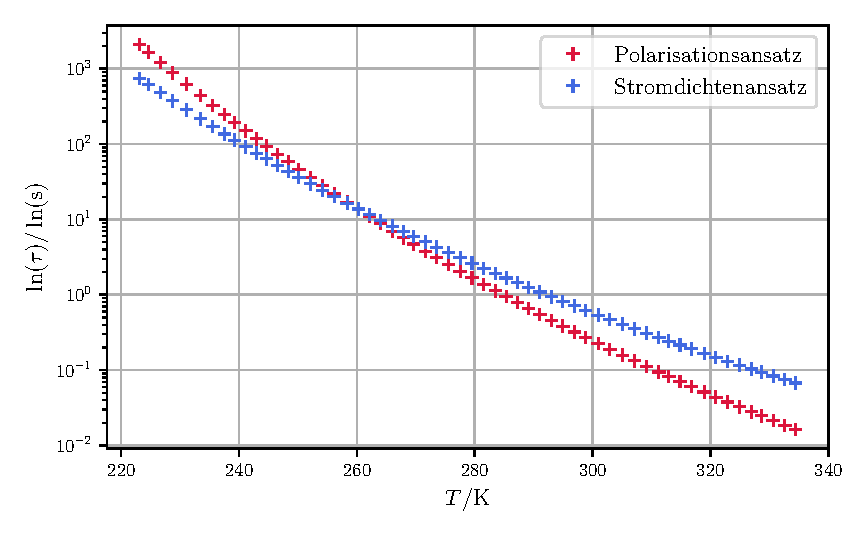
\includegraphics[width=0.8\linewidth]{scripts/build/plot1_t.pdf}
    \caption{Temperaturabhängigkeit der Relaxationszeit der ersten Messung.}
    \label{fig:t1}
\end{figure}
\begin{figure}
    \centering
    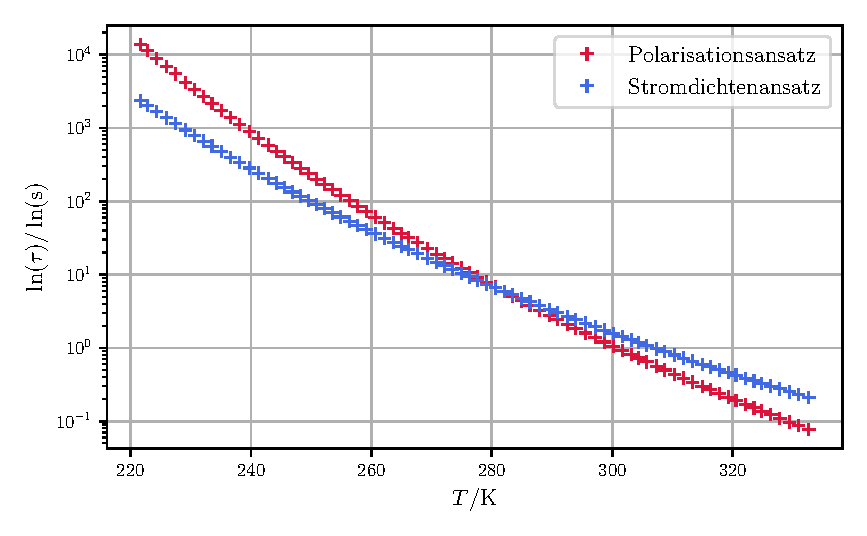
\includegraphics[width=0.8\linewidth]{scripts/build/plot2_t.pdf}
    \caption{Temperaturabhängigkeit der Relaxationszeit der zweiten Messung.}
    \label{fig:t2}
\end{figure}